\documentclass{article}

\author{Tran Van Tan Khoi}

\title{Weekly Homework Report \#5}

\date{April 16, 2025}

\usepackage[T1]{fontenc}
\usepackage[utf8]{inputenc}
\usepackage[a4paper,top=2cm,bottom=2cm,left=3cm,right=3cm,marginparwidth=1.75cm]{geometry}
\usepackage[colorlinks=true, allcolors=blue]{hyperref}
\usepackage{graphicx}
\usepackage{listings}

\lstset{language=C++,keywordstyle={\bfseries \color{blue}}}

\begin{document}

\maketitle

\section{Introduction}
\label{introduction}

This report will discuss on the \lstinline{stack} and \lstinline{queue} data structures, notably their features and implementations.

Find all source codes and documentations of this week and previous weeks in this \href{https://github.com/xtrkoi/throwaway-rep}{Github repository}.


\begin{figure*}[h]
    \centering
    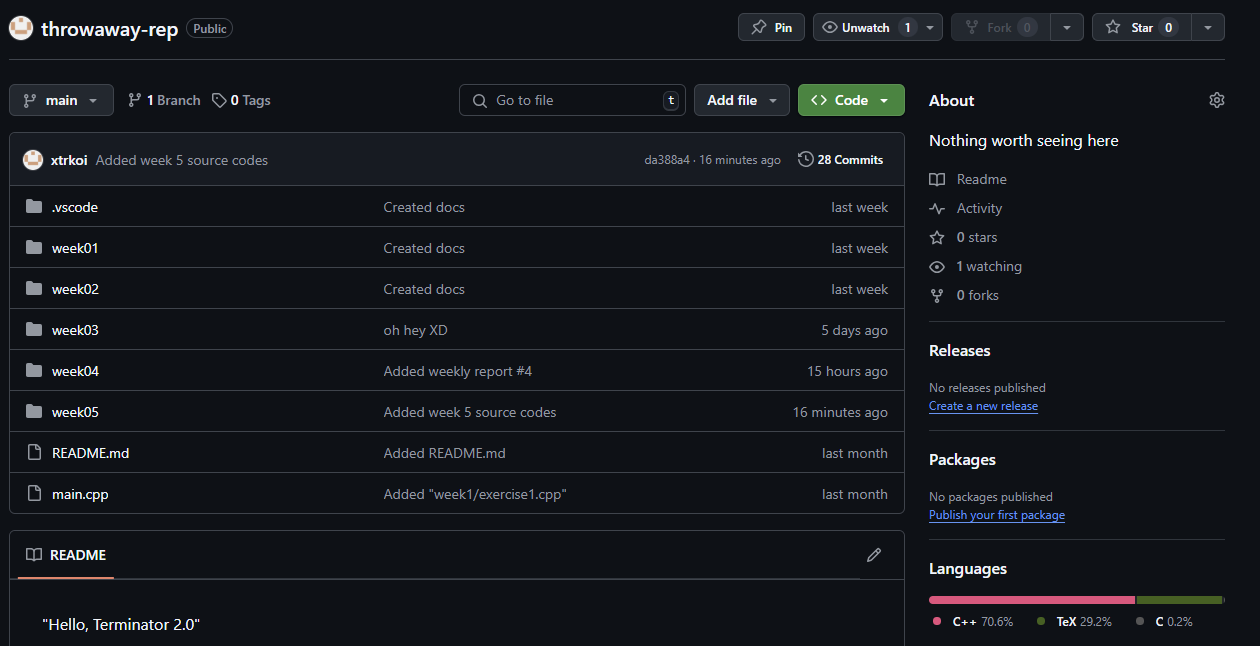
\includegraphics[width=12cm]{images/image.png}
\end{figure*}


\section{Stack}
\label{stack}

Stack is a data structure that manages data (which will be referred to as objects) linearly, from top to bottom, and dynamically. A stack keeps objects in the order of entering the stack. Typically, the first object entering the stack situates at the bottom of the stack, and the last on the top, which will be referred to as the stack's \lstinline{top}. When retrieving data from the stack, the latest data will be retrieved first, then working downward to the oldest data at the bottom. This is usually described as the Last-In-First-Out (LIFO) design pattern.

A stack has three basic functions: \lstinline{push} an object to the top, \lstinline{peek} at the top object of the stack, and \lstinline{pop} (removing) the top object of the stack. A \lstinline{size} determining function would also help in many cases. Each object in the stack does not have to follow any rule or have any certain property for the stack to work. However, modify the stack's internal structure can cause problems and is usually forbidden in implementations. If such a need for modifying the stack's internal arises then using a more advanced data structure is recommended.

The C++ STL \lstinline{std::stack} uses \lstinline{std::deque} and specifically, a double ended queue of chunks of memory, as the underlying container. However, the Linked List data structure does support adding, removing, and accessing the front (or back) object in constant time, which is suitable for being used as the underlying container for the stack in this project. Most linked list's functionalities aren't needed and we only need a method to insert a node at the front, removing the node at the front, accessing the front node, keep track of the number of nodes for constant time accesses; and a way to traverse the list for debugging purposes.

\section{Queue}
\label{queue}

A queue behaves similarly to a stack, keeping objects of data in a line from left to right dynamically, with the front at one end and the back at the other. The order of the objects is also determined by the order of entering the queue, with the oldest object at front and the lastest at the back. The oldest data will be retrieved first in this case, following the First-In-First-Out (FIFO) design pattern.

A queue also has three basic functions: \lstinline{push} (inserting) an object at the back, \lstinline{peek} at object at the front, and \lstinline{pop} (removing) the front object.

Linked list can also be used in the implementation of a queue.


\end{document}